% -*- root: ../../main.tex -*-
\section{Obiettivi e Requisiti}
	L'implementazione che si intende realizzare mira allo sviluppo di un sistema che simuli un ambiente distribuito in cui $n$ server utilizzano l'algoritmo RAFT per raggiungere il consenso. In particolare si è deciso di utilizzare, come scenario, quello di un client che contatta i server per effettuare delle \textbf{ operazioni sul database dei conti correnti bancari}.
	\begin{itemize}
			\item \textbf{Richieste del client:} il client deve poter sottomettere ai server delle operazioni da eseguire sul database dei conti corrente. Le operazioni consentite saranno:
				\begin{itemize}
					\item \emph{Deposito}
					\item \emph{Prelievo}
					\item \emph{Saldo}
				\end{itemize}
			\item \textbf{Gestione lato server:} i server devono gestire le richieste provenienti dal client e rispondere con un risultato contenente l'esito dell'operazione e il \textbf{saldo} dopo che questa è stata effettuata.
			\item \textbf{Replicazione database:} il database dei conti correnti deve essere replicato su tutti i server in maniera tale che questi ultimi eseguano \textbf{le stesse identiche istruzioni nello stesso identico ordine} ottenendo il \textbf{medesimo risultato}.
		\end{itemize}

	Il sistema dovrà inoltre rispettare requisiti che riguardano la visualizzazione delle informazioni rilevanti e l'interazione con l'utente.


	\subsection{Requisiti di visualizzazione}
	All'utente dovrà essere dato un feedback dell'avanzamento delle operazioni, per questi motivi dovranno essere visualizzate le seguenti informazioni: 
		\begin{itemize}
			\item \textbf{Ruolo:} per ciascun server bisognerà mostrare il ruolo che esso ricopre in un dato momento. I ruoli possibili sono:
				\begin{itemize}
					\item \emph{Leader (0-1)}
					\item \emph{Candidate (0-n)}
					\item \emph{Follower(0-n)}
				\end{itemize}
			\item \textbf{Ultimo commit:} l'indice dell'ultima \textbf{entry} che è stata \textbf{committata} da ciascun server.
			\item \textbf{Term corrente:} il term in cui si trova correntemente ognuno dei server.
			\item \textbf{Log:} dovrà essere visibile lo stato dei log di ciascun server affinchè si possano seguire le fasi che portano al raggiungimento del consenso e valutare se l'implementazione ricalca correttamente l'algoritmo. Ogni log è costituito da \textbf{entry}; per ogni entry si vogliono visualizzare le seguenti informazioni:
				\begin{itemize}
					\item \textbf{Term:} si tratta del \textbf{term} in cui si trovava il \textbf{leader} che ha creato l'entry, nel momento in cui questa è stata generata. 
					\item \textbf{Comando:} l'\textbf{operazione da eseguire}, contenuta nella richiesta del client 
					\item \textbf{Indice:} la \textbf{posizione} di quella determinata \textbf{entry} all'interno del log del relativo server.
					\item \textbf{Stato:} se l'\textbf{entry} è \textbf{committed} o meno. Se una entry è committed, non dovrà in alcun modo essere possibile che ne compaia una non committata con indice precedente ad essa.
				\end{itemize} 
			\item \textbf{Stato di esecuzione:} dovrà esserci la possibilità di visualizzare le richieste sottomesse dal client e, per ognuna di esse, capire se essa è \textbf{già stata eseguita}
			\item \textbf{Risultati:} nel caso in cui una richiesta del client sia stata eseguita, sarà necessario mostrare all'utente il risultato relativo, ricevuto dal client. Esso \textbf{non dovrà differire} dai risultati ottenuti su ciascuno dei server.
		\end{itemize}

	\subsection{Requisiti di interazione}
	L'applicativo dovrà avere un'interfaccia utente che permetta di interagire con il sistema agendo su determinati parametri. I modi in cui il sistema potrà essere manovrato dall'utente sono i seguenti:
		\begin{itemize}
			\item \textbf{Operazione:} dovrà essere reso disponibile un modo per \textbf{effettuare una richiesta} (da parte del client) a uno dei server.
			\item \textbf{Stop/Resume:} il comando \textit{stop} servirà per simulare la temoranea assenza di un server, mentre il comando \textit{resume} ne farà ripartire l'attività. 
			\item \textbf{Perdita dei messaggi:} l'utente potrà impostare una percentuale di perdita di messaggi per ogni server, in maniera indipendente. Questa funzionalità permetterà di testare la resistenza a questo tipo di fault.
			\item \textbf{Timer:} sarà possibile provocare lo scadere del timer. Tale azione assumerà significati di versi a seconda del ruolo che il server ricoprirà in quel momento:
				\begin{itemize}
					\item \textbf{Leader:} lo scadere del timer porterà all'invio degli heartbeat.
					\item \textbf{Candidate:} la scadenza del timer lo porterà ad aumentare il proprio term e ricandidarsi
					\item \textbf{Follower:} allo scattare del timer, il follower, non avendo ricevuto notizie dal leader, deciderà di aumentare il proprio term e cambiare il proprio stato in \textit{candidate}.
				\end{itemize}

		\end{itemize}


\begin{figure}[H]
  \centering
  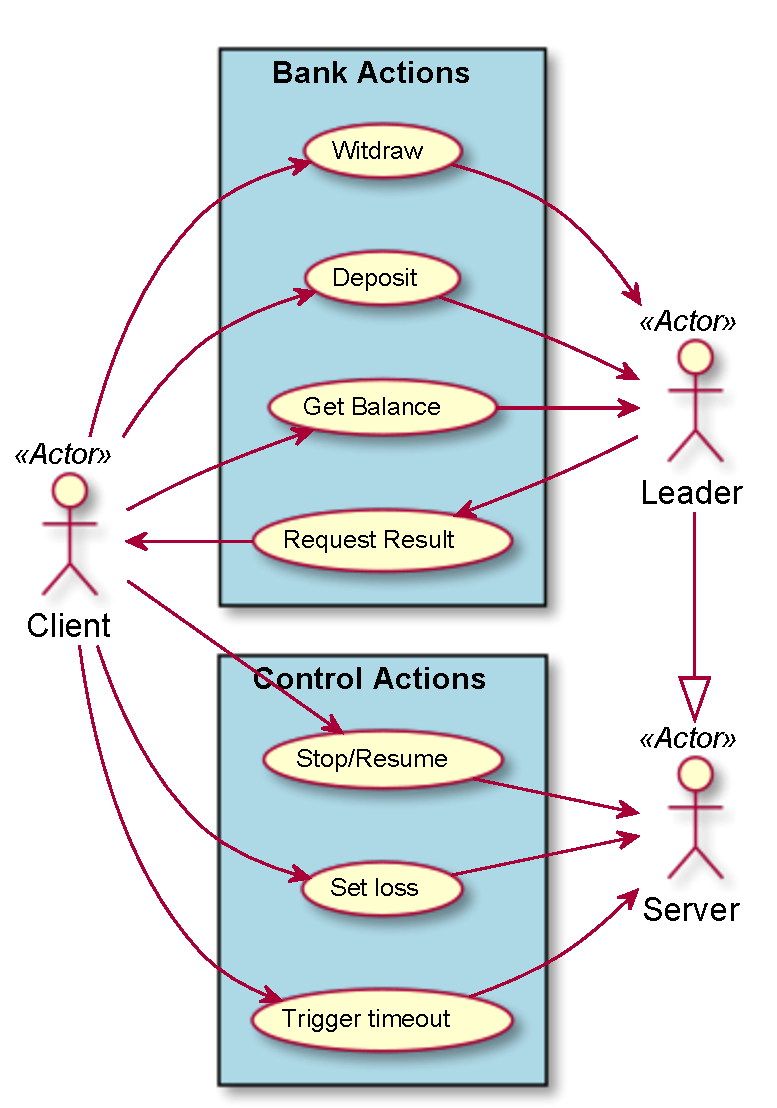
\includegraphics[width=0.99\columnwidth]{useCaseDiagrams/useCaseDiagram}
  \caption[useCaseDiagramCaption]{}
  
  \label{fig:figure28}
\end{figure}